\section{Evaluation Lösungsprinzipien}

Aus der vorhergehenden Technologierecherche wird pro Studiengang ein morphologischer Kasten erstellt. Dieser wird befüllt mit den Teilfunktionen und den recherchierten Technologien. Damit werden die Lösungsprinzipien evaluiert und verschiedene Varianten werden ausarbeitet. Nachfolgend sind alle morphologischen Kästen aufgezeigt.

Die Lösungsvarianten wurden gewaählt anhand der Muss-Kriterien, die erreicht werden sollen: Simpel, nicht zu teuer, nicht die 30cmx30cmx80cm ausnutzen, Robustheit. Zusätzlich wurde in Betracht gezogen, wie stimmig die einzelnen Technologien miteinander sind.

\subsection{Mechanik Morphologischer Kasten}

Auf Basis der Technologierecherche wurden verschiedene Lösungsansätze für die einzelnen Teilfunktionen ausgewählt und in den morphologischen Kasten aufgenommen.

\begin{itemize}
    \item Variante A - Gelb: Zwei von drei Rädern werden direkt durch einen Motor angetrieben. Das dritte Rad ist frei drehend und dient als Stützrad. Das Hindernis wird mit einem parallel Greifer angehoben. Da Variante A nur drei Räder hat bietet sich eine U-Form für das Chassis an. 
    \item Variante B - Rot: Die vier Räder sind diamantförmig angeordnet. Zwei Räder werden direkt angetrieben, die weiteren Räder sind frei drehende Stützräder. Der Greifer ist an einem Arm befestigt. 
    \item Variante C - Grün: Die Fortbewegung erfolgt mit zwei separat angesteuerten Raupen. Angesteuert werden die Raupen durch ein Überlagerungsgetriebe. Das Hindernis wird mit einem Gabelgreifer angehoben. 
\end{itemize}

\begin{table}[H]
\centering
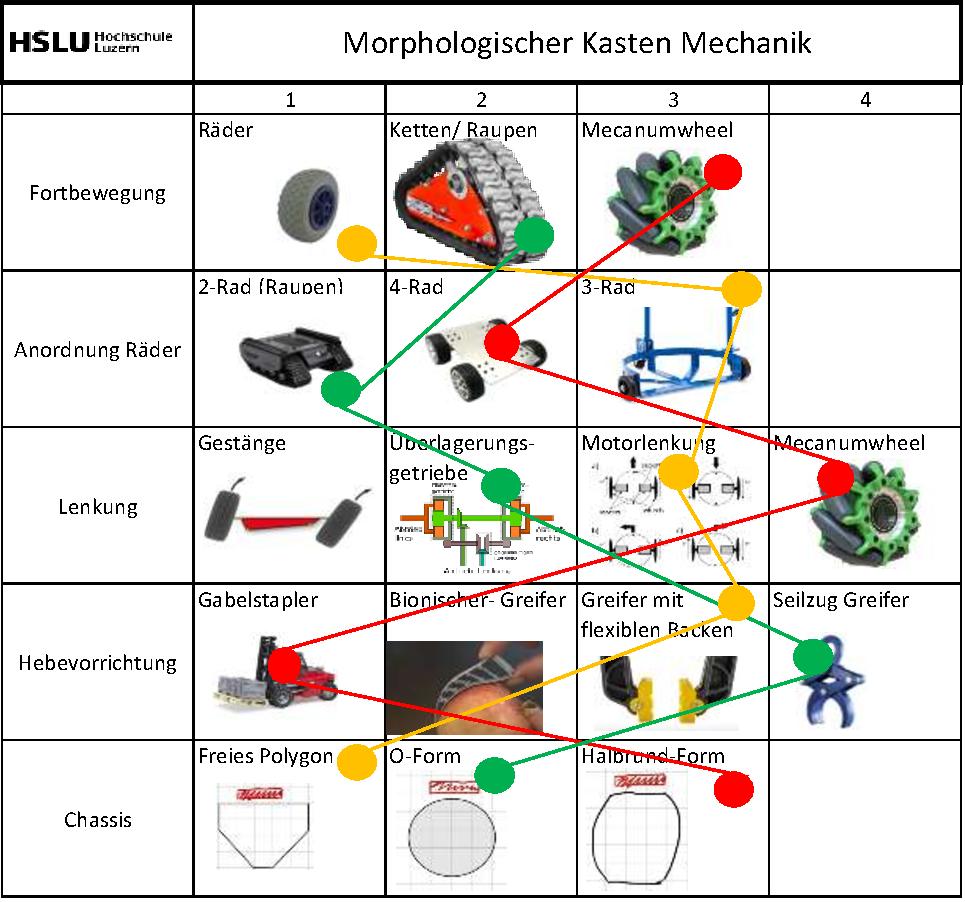
\includegraphics[width=\textwidth]{assets/MK_Maschinentechnik.pdf}
\caption{Morphologischer Kasten: Mechanik}
\label{table:mk-mechanik}
\end{table}


\subsection{Steuerung Morphologischer Kasten}

Aus der Technologierecherche entstand folgender morphologischer Kasten mit drei Varianten für die Teilfunktionen, die die Elektronik und die Steuerung im Roboter bilden.

\begin{itemize}
    \item Variante A - Gelb: Das verwenden vom Tiny K22 macht das System echtzeitfähig. Leichte Motoren werden eingesetzt. Inputs und Outputs werden einfach gehalten über Leuchten und Schalter. Für die Motorsteuerug werden die Treiber eingekauft.
    \item Variante B - Rot: Bei dieser Variante werden die Bauteile Raspberry Pi tauglich verwendet, grob gesagt eine "Plug and Play" Methode. Ebenfalls haben die Motoren ein geringes Gewicht.
    \item Variante C - Grün: Durch die Schrittmotoren und die Objekterkennung mit Lidar weist diese Kombination eine hohe Präzision auf. Mit dem Horn als akustisches Signal wäre dieser Komponent auffällig und einzigartig. Aufgrund der Schrittmotoren wird der Roboter schwer, was ein Nachteil ist.
\end{itemize}

\begin{table}[H]
\centering
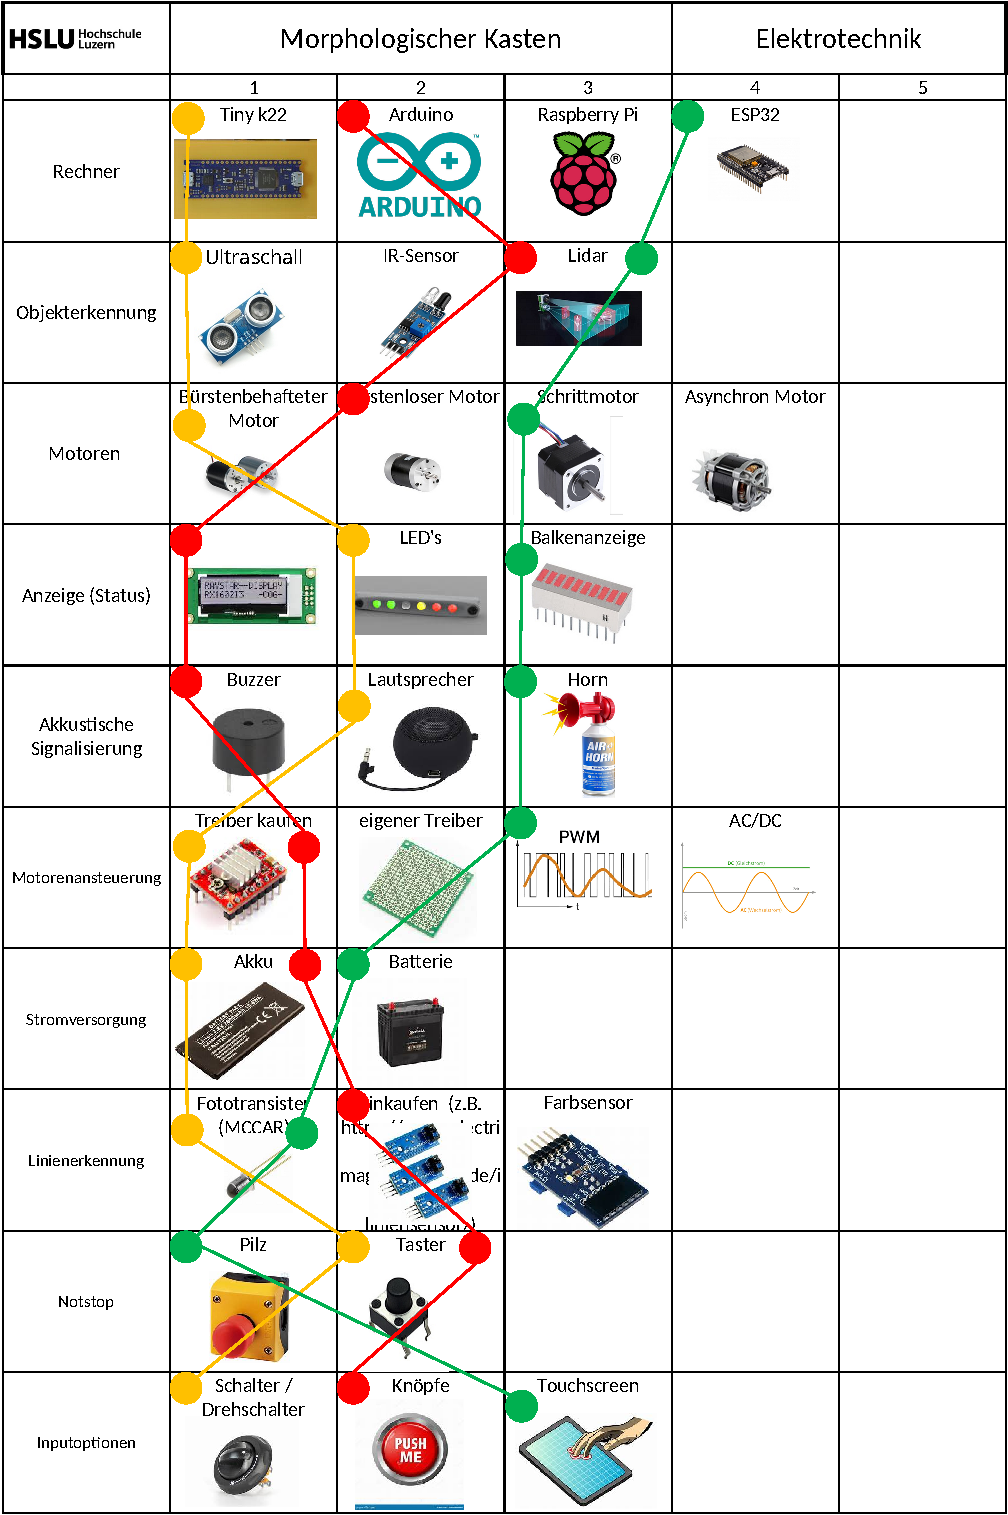
\includegraphics[width=\textwidth -5mm]{assets/MK_Elektrotechnik.pdf}
\caption{Morphologischer Kasten: Steuerung}
\label{table:mk-elektrotechnik}
\end{table}

In allen drei Varianten ist konsequent ein Mikrocontroller vorgesehen. Einige Komponenten, wie etwa Buzzer und Lautsprecher oder Drehschalter und Tasten, sind grösstenteils austauschbar. Spezifische Schaltungselemente wie Strombegrenzer und Spannungsregler wurden hingegen nicht im morphologischen Kasten berücksichtigt, da solche Entscheidungen erst während des Layoutprozesses getroffen werden.


\subsection{Navigation Morphologischer Kasten}

Aus der Technologierecherche wurde folgender morphologischer Kasten mit drei Varianten für die Teilfunktionen, die die Navigation bilden, erstellt.

\begin{itemize}
     \item Variante A - Gelb: Python verwendet eine Mischung aus PyTorch und OpenCV, um AI und reine Bilderkennung zu verwenden. Dijkstra berechnet den Weg. Das Ganze rechnet auf einem Raspberry Pi mit einer Raspberry Camera angeschlossen. Diese Methode ist robust, da zwei Moeglichkeiten zur Erkennung des Graphes verwednet werde nkoennen. Die Kamera und das Board passen gut zusammen und sind recht guenstig. 
    \item  Variante B - Rot: Python verwendet LiteRT, um mit AI die Umgebung zu erkennen und Dijkstra, um den Weg zu berechnen. Das Ganze rechnet auf einem Coral Dev Board und fotografiert den Graphen mit einer Industriekamera. Mit Tensorflow koennte sicher alles erkannt werden. Jedoch ist dies auch ein relativ grosser Algorithmus. Das Coral Dev Board ist staerker als ein Raspberry Pi aber auch teurer.
    \item Variante C - Grün: Python verwendet nur OpenCV zur Bilderkennung und berechnet mit Dijkstra den Weg, es rechnet auf einem Raspberry Pi mit einer Raspberry Camera. Diese Variante koennte schwierig werden, da moeglicherweise nicht alle Elemente erkannt werden koennen.
\end{itemize}

\begin{table}[H]
\centering
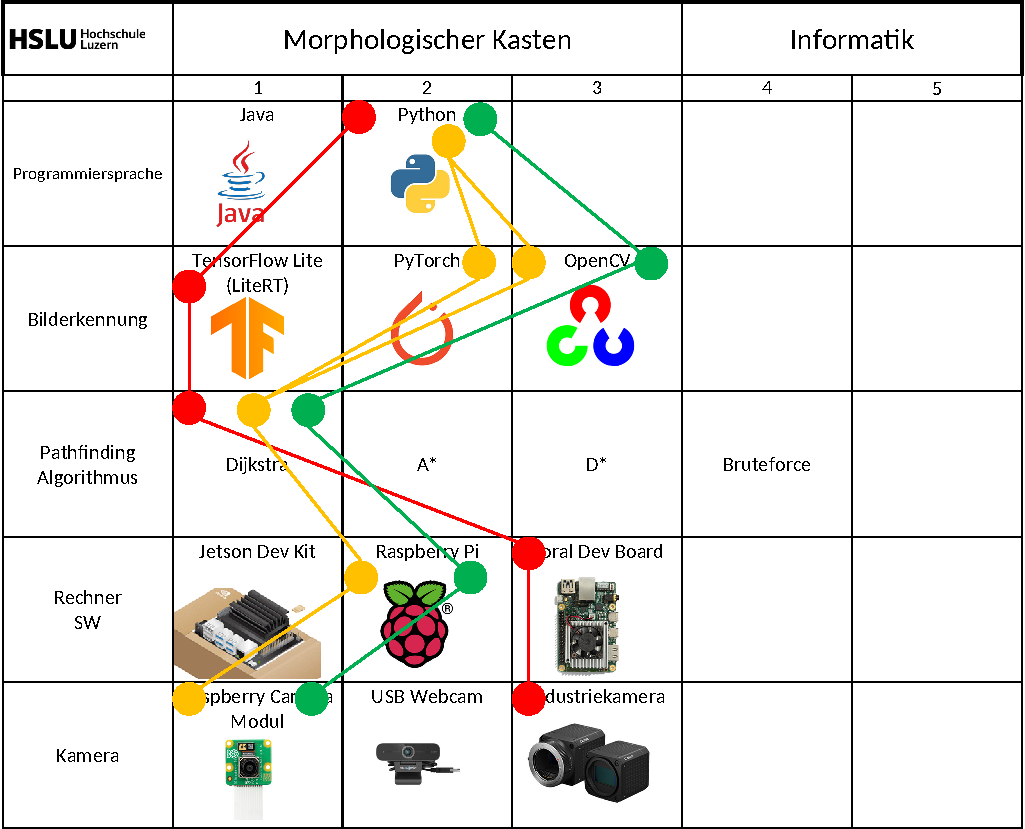
\includegraphics[width=\textwidth]{assets/MK_Informatik.pdf}
\caption{Morphologischer Kasten: Navigation}
\label{table:mk-informatik}
\end{table}


Bei den drei Varianten fällt auf, dass alle Python und den Wegfindealgorithmus Dijkstra verwenden. Python wurde immer gewählt, da Bilderkennung und Machine Learning sehr gut mit Python harmonisieren. Viele Libraries, inklusive dieser, die hier ersichtlich sind, sind kompatibel mit Python. Dijkstra wurde immer gewählt, weil dieser Algorithmus simpel und robust ist und die Geschwindigkeit vernachlässigbar ist. Da es im Graphen nur 8 Knoten gib, wird die Berechnung bei jedem Algorithmus schnell sein.

\subsection{Simulator Morphologischer Kasten}


Aus der Technologierecherche wurde folgender Morphologischer Kasten für die Teilfunktonen des Simulators erstellt. Es gibt drei Varianten, die in Frage kommen.

\begin{table}[H]
\centering
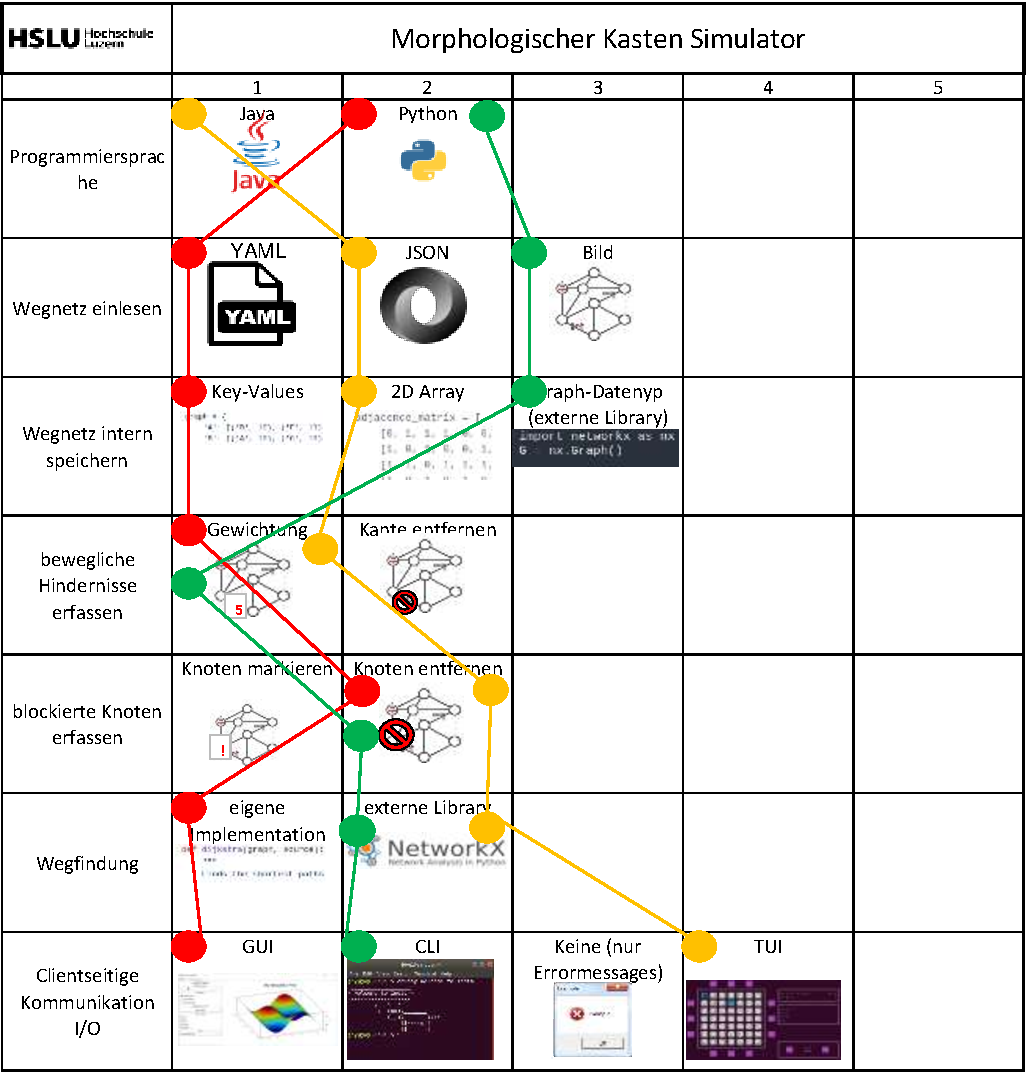
\includegraphics[width=\textwidth]{assets/MK_Simulator.pdf}
\caption{Morphologischer Kasten: Simulator}
\label{table:mk-simulator}
\end{table}



Beim Erfassen von beweglichen Hindernissen wird in jeder Lösungsvariante die Kante nicht entfernt, sondern neu gewichtet. Es ist nicht garantiert, dass es immer einen Weg ohne beweglichem Hinderniss gibt. Diese Strecken zu entfernen, wäre zu risikobehaftet.

Ebenfalls wird ein Knoten immer entfernt falls ein Pylon darauf steht. Er wird nicht markiert, da es würde keinen Vorteil bringen, den Knoten weiterhin zu speichern.


\newpage
\section{Auswahl Lösungskombinationen}

Zur Auswahl der passendsten Lösungskombination wird pro Teilbereich eine Nutzwertanalyse durchgeführt. Die Kriterien und deren Gewichtung sind individuell pro Teilbereich, damit sie ideal passen. Die Variante mit der höchsten Punktezahl ist die Variante, die am besten passt.

\subsection{Mechanik Nutzwertanalyse}

Folgende drei Lösungskombinationen aus dem morphologischen Kasten werden in der Nutzwertanalyse untersucht. 



\begin{table}[H]
\centering
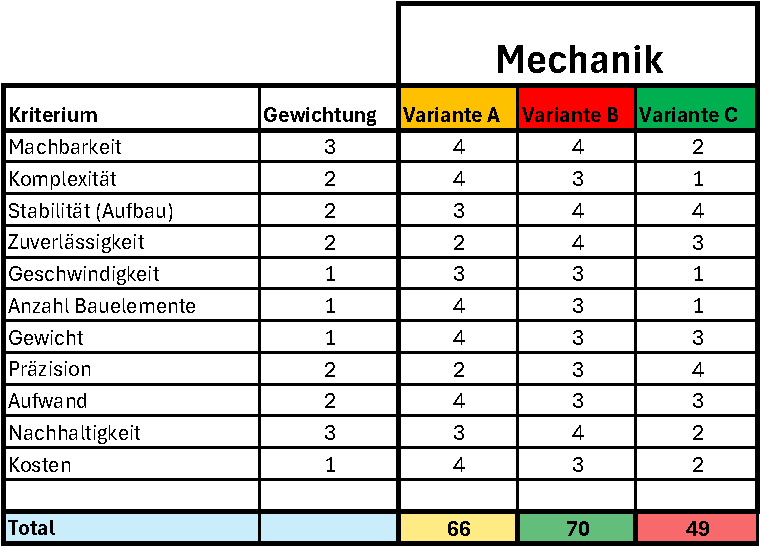
\includegraphics[width=0.75\textwidth]{assets/Nutzwertanalyse-M.pdf}
\caption{Nutzwertanalyse: Maschinentechnik}
\label{table:nutzwert-maschinentechnik}
\end{table}

Die Analyse der drei genannten Varianten hat ergeben, dass die Variante C sich am besten für die Umsetzung eignet. Enstprechend wurden folgende Komponenten und Systeme ausgewählt. 

\begin{itemize}
    \item Fortbewegung: Räder 
    \item Anordnung:  Zwei Räder hinten und ein Stützrad vorne
    \item Lenkung: Direkt Antrieb für zwei Räder
    \item Hebevorrichtung: Parallele Greifer Backen
    \item Chassis: U-Form 
\end{itemize}

\subsection{Steuerung Nutzwertanalyse}

Mithilfe des morphologischen Kastens wurden verschiedene Lösungsvarianten aufgezeigt. Die Varianten bestehen aus diversen Komponenten. 



\begin{table}[H]
\centering
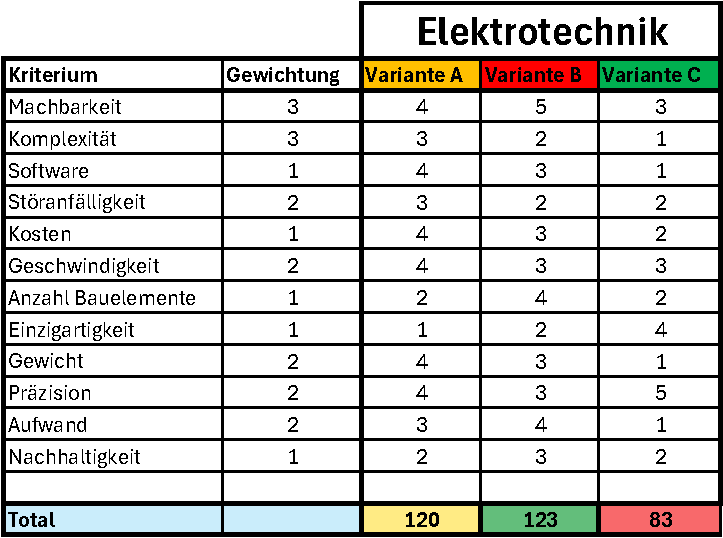
\includegraphics[width=0.75\textwidth]{assets/Nutzwertanalyse-ET.pdf}
\caption{Nutzwertanalyse: Elektrotechnik}
\label{table:nutzwert-ET}
\end{table}

Aus den Bewertungen aus der Nutzwertanalyse zeigt sich die Variante A als höchst bewertete. Somit wird diese Variante weiter verfolgt und besteht aus folgenden Komponenten.

\begin{itemize}
    \item Rechner: Tiny K22
    \item Objekterkennung: Ultraschall
    \item Motoren: Bürstenbehafteter Motor
    \item Anzeige: LEDs 
    \item Akkustische Signalisierung: Lautsprecher
    \item Motorenansteuerung: Treiber einkaufen
    \item Stromversorgung: Akku
    \item Linienerkennung: Fototransistor
    \item Not-Stop: Taster
    \item Inputoption: Schalter
\end{itemize}

\subsection{Navigation Nutzwertanalyse}

Die drei ermittelten Varianten aus dem vorherigen Kapitel werden analysiert und bewertet mithilfe einer Nutzwertanalyse.


\begin{table}[H]
\centering
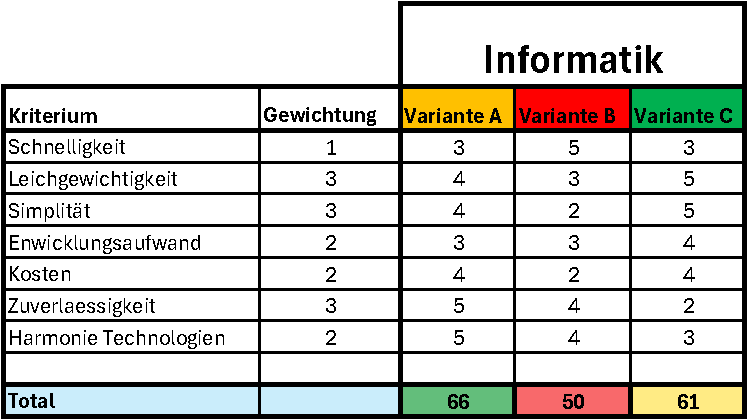
\includegraphics[width=0.75\textwidth]{assets/Nutzwertanalyse-I.pdf}
\caption{Nutzwertanalyse: Informatik}
\label{table:nutzwert-informatik}
\end{table}

Aus der Nutzwertanalyse kann abgelesen werden, dass die Variante A mit Python, PyTorch und OpenCV am besten passt. Die entsprechenden Komponenten aus dieser Variante sind nachfolgend aufgelistet.

\begin{itemize}
    \item Programmiersprache: Python
    \item Bilderkennung: PyTorch und OpenCV
    \item Pathfinding Algorithmus: Dijkstra
    \item Rechner SW: Raspberry Pi
    \item Kamera: Raspberry Camera Modul
\end{itemize}

\subsection{Simulator Nutzwertanalyse}

Die drei Varianten wie der Simulator umgesetzt werden könnte, werden bewertet in folgender Nutzwertanalyse. Die Kriterien und deren Gewichtung sind dieselben, wie bei der Nutzwertanalyse für die Informatik im Roboter. Das Ziel des Simulators ist es, diesen möglichst realistisch und wiederverwendbar für \acrshort{pren2} umzusetzen.


Die folgenden drei Lösungskombinationen, werden im nächsten Schritt evaluiert.

\begin{itemize}
    \item Variante A: Ein Java Simulator liest ein JSON File und speichert es in einem 2D Array. Bei einem beweglichen Hindernis wird die Gewichtung der Kante erhöht, bei einem Pylonen wird der Knoten entfernt. Dijkstra wird mit einer externen Library implementiert. Die Auswahl des Zielknotens erfolgt zufällig und die Aktivitäten des Roboters werden in einem TUI dargestellt.
    \item Variante B: Ein Python Simulator liest ein YAML File und speichert es in einem Dictionary. Bei einem beweglichen Hindernis wird die Gewichtung der Kante erhöht, bei einem Pylonen wird der Knoten entfernt. Dijkstra wird selber implementiert, das Ziel kann vom Menschen und zufällig ausgewählt werden und die Aktivitäten des Roboters sind in einem GUI ersichtlich.
    \item Variante C: Ein Python Simulator liest ein Bild ein und speichert es in einem Graph Datentyp. Bei einem beweglichen Hindernis wird die Gewichtung der Kante erhöht, bei einem Pylonen wird der Knoten entfernt. Eine externe Library implementiert Dijkstra, das Ziel wird manuell ausgwählt und die Aktivitäten des Roboters werden in einem CLI dargestellt.
\end{itemize}

\begin{table}[H]
\centering
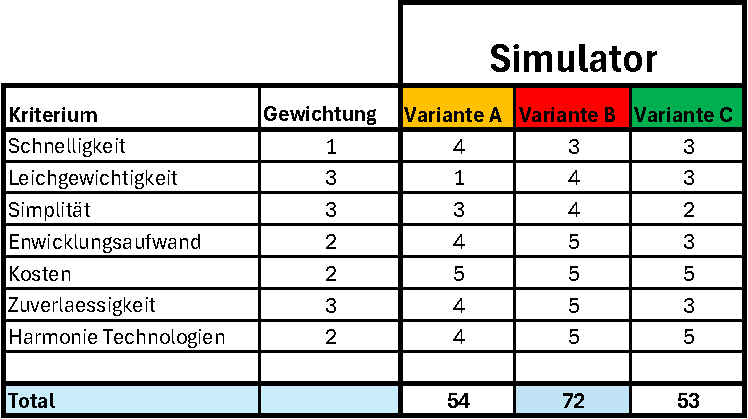
\includegraphics[width=0.75\textwidth]{assets/Nutzwertanalyse-Simulator.pdf}
\caption{Nutzwertanalyse: Simulator}
\label{table:nutzwert-Simulator}
\end{table}

Die Nutzwertanalyse zeigt, dass die Variante B: Python mit YAML und einem GUI am besten abschneidet. Diese Variante besteht aus folgenden Teilen.

\begin{itemize}
    \item Programmiersprache: Python
    \item Wegnetz einlesen: YAML
    \item Wegnetz intern speichern: Key-Values
    \item Bewegliche Hindernisse erfassen: Gewichtung
    \item Blockierte Knoten erfassen: Knoten entfernen
    \item Wegfindung: eigene Implementation
    \item Zielauswahl: human input und random
    \item Clientseitige Kommunikation I/O: GUI
\end{itemize}